
%%--------------------------------------------------
%% Holt: Multiple Choice Questions
%%--------------------------------------------------


%% Chapter 06: Momentum and Collisions
%%--------------------------------------------------


%% Holt Multiple Choice Questions
%%--------------------------------------------------
\element{holt-mc}{
\begin{question}{holt-ch06-Q01}
    If a particle's kinetic energy is zero,
        what is its momentum?
    \begin{multicols}{2}
    \begin{choices}
      \correctchoice{zero}
        \wrongchoice{\SI{1}{\kilo\gram\meter\per\second}}
        \wrongchoice{\SI{15}{\kilo\gram\meter\per\second}}
        \wrongchoice{negative}
    \end{choices}
    \end{multicols}
\end{question}
}

\element{holt-mc}{
\begin{question}{holt-ch06-Q02}
    The vector below represents the momentum of a car
        traveling along a road.
    \begin{center}
    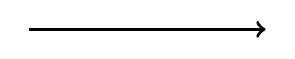
\begin{tikzpicture}
        \draw[very thick,->] (0,0) -- (3,0);
    \end{tikzpicture}
    \end{center}
    The car strikes another car,
        which is at rest,
        and the result is an inelastic collision.
    Which of the following vectors represents the momentum of
        the first car after the collision?
    \begin{multicols}{2}
    \begin{choices}
        \wrongchoice{
            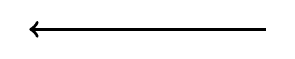
\begin{tikzpicture}
                \draw[very thick,->] (3,0) -- (0,0);
            \end{tikzpicture}
        }
        \wrongchoice{
            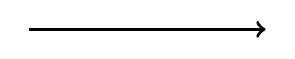
\begin{tikzpicture}
                \draw[very thick,->] (0,0) -- (3,0);
            \end{tikzpicture}
        }
        \wrongchoice{
            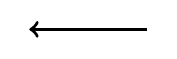
\begin{tikzpicture}
                \draw[very thick,->] (1.5,0) -- (0,0);
            \end{tikzpicture}
        }
        \correctchoice{
            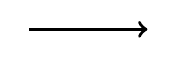
\begin{tikzpicture}
                \draw[very thick,->] (0,0) -- (1.5,0);
            \end{tikzpicture}
        }
    \end{choices}
    \end{multicols}
\end{question}
}

\element{holt-mc}{
\begin{question}{holt-ch06-Q03}
    What is the momentum of a \SI{0.148}{\kilo\gram} baseball
        thrown with a velocity of \SI{35}{\meter\per\second} toward home plate?
    \begin{choices}
        \wrongchoice{\SI{5.1}{\kilo\gram\meter\per\second} toward home plate}
        \wrongchoice{\SI{5.1}{\kilo\gram\meter\per\second} away from home plate}
      \correctchoice{\SI{5.2}{\kilo\gram\meter\per\second} toward home plate}
        \wrongchoice{\SI{5.2}{\kilo\gram\meter\per\second} away from home plate}
    \end{choices}
\end{question}
}

\element{holt-mc}{
\begin{question}{holt-ch06-Q04}
    After being struck by a bowling ball,
        a \SI{1.5}{\kilo\gram} bowling pin slides to the right at
        \SI{3.0}{\meter\per\second} and collides head-on with
        another \SI{1.5}{\kilo\gram} bowling pin initially at rest.
    %% Begin question
    What is the final velocity of the second pin if the first pin
        moves to the right at \SI{0.5}{\meter\per\second} after the collision?
    \begin{choices}
        \wrongchoice{\SI{2.5}{\meter\per\second} to the left}
      \correctchoice{\SI{2.5}{\meter\per\second} to the right}
        \wrongchoice{\SI{3.0}{\meter\per\second} to the left}
        \wrongchoice{\SI{3.0}{\meter\per\second} to the right}
    \end{choices}
\end{question}
}

\element{holt-mc}{
\begin{question}{holt-ch06-Q05}
    After being struck by a bowling ball,
        a \SI{1.5}{\kilo\gram} bowling pin slides to the right at
        \SI{3.0}{\meter\per\second} and collides head-on with
        another \SI{1.5}{\kilo\gram} bowling pin initially at rest.
    %% Begin question
    What is the final velocity of the second pin if the first pin
        stops moving when it hits the second pin?
    \begin{choices}
        \wrongchoice{\SI{2.5}{\meter\per\second} to the left}
        \wrongchoice{\SI{2.5}{\meter\per\second} to the right}
        \wrongchoice{\SI{3.0}{\meter\per\second} to the left}
      \correctchoice{\SI{3.0}{\meter\per\second} to the right}
    \end{choices}
\end{question}
}

\element{holt-mc}{
\begin{question}{holt-ch06-Q06}
    For a given change in momentum,
        if the net force that is applied to an object increases,
        what happens to the time interval over which the force is applied?
    \begin{choices}
      \correctchoice{The time interval increases.}
        \wrongchoice{The time interval decreases.}
        \wrongchoice{The time interval stays the same.}
        \wrongchoice{It is impossible to determine the answer from the given information.}
    \end{choices}
\end{question}
}

\element{holt-mc}{
\begin{question}{holt-ch06-Q07}
    Which equation expresses the law of conservation of momentum?
    \begin{choices}
        \wrongchoice{$\mathbf{p} = m\mathbf{v}$}
      \correctchoice{$m_1\mathbf{v_{1,i}} + m_2 \mathbf{v_{2,i}} = m_1 \mathbf{v_{1,f}} + m_2 \mathbf{v_{2,f}}$}
        \wrongchoice{$\frac{1}{2} m_1 v_{1,i}^2 + m_2 v_{2,i}^2 = \frac{1}{2} \left( m_1 + m_2 \right) v_f^2$}
        \wrongchoice{$KE = \mathbf{p}$}
    \end{choices}
\end{question}
}

\element{holt-mc}{
\begin{question}{holt-ch06-Q08}
    Two shuffleboard disks of equal mass,
        one of which is orange and one of which is yellow,
        are involved in an elastic collision.
    The yellow disk is initially at rest and is struck by the orange disk,
        which is moving initially to the right at \SI{5.00}{\meter\per\second}.
    After the collision, the orange disk is at rest.
    What is the velocity of the yellow disk after the collision?
    \begin{choices}
        \wrongchoice{zero}
        \wrongchoice{\SI{5.00}{\meter\per\second} to the left}
        \wrongchoice{\SI{2.50}{\meter\per\second} to the right}
      \correctchoice{\SI{5.00}{\meter\per\second} to the right}
    \end{choices}
\end{question}
}

\newcommand{\holtChSixQNine}{
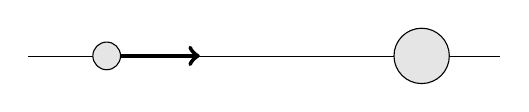
\begin{tikzpicture}
    \draw[very thin] (-3,0) -- (3,0);
    \node[draw,circle,fill=white!90!black,minimum size=1em] (A) at (-2,0) {};
    \node[draw,circle,fill=white!90!black,minimum size=2em] (B) at (+2,0) {};
    \draw[ultra thick,->] (A.east) -- ++(0:1cm);
\end{tikzpicture}
}

\element{holt-mc}{
\begin{question}{holt-ch06-Q09}
    A \SI{0.400}{\kilo\gram} bead slides on a straight frictionless wire and moves with a velocity of \SI{3.50}{\centi\meter\per\second} to the right,
        as shown below.
    \begin{center}
        \holtChSixQNine
    \end{center}
    The bead collides elastically with a larger \SI{0.600}{\kilo\gram} bead that is initially at rest.
    After the collision, the smaller bead moves to the left with a velocity of \SI{0.70}{\meter\per\second}.
    %% Begin Qeustion
    What is the large bead's velocity after the collision?
    \begin{choices}
        \wrongchoice{\SI{1.68}{\centi\meter\per\second} to the right}
        \wrongchoice{\SI{1.87}{\centi\meter\per\second} to the right}
      \correctchoice{\SI{2.80}{\centi\meter\per\second} to the right}
        \wrongchoice{\SI{3.97}{\centi\meter\per\second} to the right}
    \end{choices}
\end{question}
}

\element{holt-mc}{
\begin{question}{holt-ch06-Q10}
    A \SI{0.400}{\kilo\gram} bead slides on a straight frictionless wire and moves with a velocity of \SI{3.50}{\centi\meter\per\second} to the right,
        as shown below.
    \begin{center}
        \holtChSixQNine
    \end{center}
    The bead collides elastically with a larger \SI{0.600}{\kilo\gram} bead that is initially at rest.
    After the collision, the smaller bead moves to the left with a velocity of \SI{0.70}{\meter\per\second}.
    %% Begin Question
    What is the total kinetic energy of the system of beads after the collision?
    \begin{multicols}{2}
    \begin{choices}
        \wrongchoice{\SI{1.40e-4}{\joule}}
      \correctchoice{\SI{2.45e-4}{\joule}}
        \wrongchoice{\SI{4.70e-4}{\joule}}
        \wrongchoice{\SI{4.90e-4}{\joule}}
    \end{choices}
    \end{multicols}
\end{question}
}


\endinput

